\subsection{Learning equation choices for groups of targets}
\label{sec:batch-reuse}
The shared variable in Eq.~\eqref{eq:loop-shared-variable} removes repeated
reductions at different loop orders. We now reduce repeated work within
each target set and across independent mass profiles of the same restricted
vacuum family. The calculation still uses one power of every massless
denominator and \(R=2,3,4\) distinct massive denominators. Kira performs
exact elimination on the supplied Euler and partial-fraction identities,
and the retained native IBP-generation interfaces continue to serve their
previously tested two- and three-loop domains.

For a target set \(\mathcal T\), let \(\pi\) specify an ordering of the
\(R\) massive denominators. At each mixed integral, we use the first two
active denominators in this ordering in Eq.~\eqref{eq:loop-shared-mass}.
Every resulting integral has a smaller total power \(B\), and repeated
integrals share the same subsequent reduction. Let
\(\mathcal D_\pi(\mathcal T)\) be the resulting set of distinct nonmaster
integrals. To train a model that favors small shared systems, we assign
the cost
\begin{equation}
 S_\pi(\mathcal T)=
 \sum_{\boldsymbol b\in\mathcal D_\pi(\mathcal T)}
 \left(3\sum_{j=1}^{R}b_j-2\right).
 \label{eq:batch-weighted-cost}
\end{equation}
The weight increases with the number of polynomial coefficients that can
enter a substitution. It provides a training measure of algebraic work;
actual Kira operation counts and the cost of large rational numbers also
depend on its elimination and simplification choices. The smallest
\(S_\pi\) among the \(R!\) mass orderings supplies a restricted reference
for the quality of a choice. More general reduction paths can have
different costs.

We train ensembles of four and sixteen extremely randomized regression
trees~\cite{Geurts2006ExtraTrees} to predict \(\log S_\pi\), then select the
ordering with the smallest predicted value. The 32 inputs describe the
target count, number of massive denominators, total powers, the mean and mean squared power at each
position of \(\pi\), the largest power, the fraction of targets with that
denominator present, and pairwise mean minima and products of powers.
These inputs describe sharing across the entire target set. Each prediction estimates the reduction cost, while exact identities
and Kira determine the reduction coefficients. Two massive denominators admit a single pair, so those
requests bypass inference.

The training set contains 420 target batches and 6,300 candidate orderings,
with total powers up to fourteen and at most 128 targets per batch.
Both ensembles have maximum depth twelve and at least three training
examples per leaf. We compare their complete calculation times with
four simple ordering rules, the earlier learned pair selector, and
enumeration of all fixed orderings. The first validation uses 324
calculations on twelve new mass profiles and selects the four-tree
ensemble as the cheaper learned candidate. Its time ratio to the
fastest simple rule is 1.000, so single-profile deployment
retains that rule. A further 48 validation applications combine three
profiles at a time and give a learned-to-simple time ratio of
0.925, which selects learned ordering for that route.

The selected trees require 7634 nodes in total. We also store their
unchanged thresholds and leaf values in compiled inference routines to
reduce loading and prediction cost. All 12,600 compared candidate scores
agree exactly with the original tree evaluation. For the selected
ensemble, compiled evaluation takes 0.921 times the Python
decision time over the training batches. Fresh complete-calculation
validation then chooses the inference implementation used for production calculations; this comparison includes
model loading and inference and measures the time of the complete calculation.

\subsubsection{Sharing exact checks and Kira calls}
The original shared reduction still expanded and checked the same
coefficient separately at each requested loop order. We instead compare
the Kira coefficient \(C_{\boldsymbol b j}(z)\) with an independent
Taylor partial-fraction construction directly in \(\mathbb Q[z]\).
Exact equality in this polynomial ring implies equality after the
substitution \(z=L(d-2)\) for each requested \(L\). Every returned
coefficient therefore keeps an exact check while each symbolic comparison
takes place once.

We also use integer polynomial arithmetic when reading the coefficients
and applying the substitution. If
\(C(z)=D^{-1}\sum_{n=0}^{q}a_nz^n\), where the \(a_n\) are integers and
\(D\) is a positive common denominator, then the coefficient of \(d^k\)
after substitution is
\begin{equation}
 [d^k]C\bigl(L(d-2)\bigr)
 =\frac{1}{D}\sum_{n=k}^{q}a_n L^n
   \binom{n}{k}(-2)^{n-k}.
 \label{eq:batch-integer-substitution}
\end{equation}
Here \(q\) is the polynomial degree and \([d^k]\) denotes extraction of
the coefficient of \(d^k\). This form keeps the inner sums in integer
arithmetic and reduces the number of repeated fraction normalizations.
These savings follow from exact algebra, separately from the learned
choice of equations.

Independent mass profiles can also share a Kira invocation. We give each
profile its own integral identifiers and master basis, then form
\begin{equation}
 A=\operatorname{diag}(A_1,\ldots,A_P),\qquad
 A\begin{pmatrix}\boldsymbol I_1\\ \vdots\\ \boldsymbol I_P\end{pmatrix}
 =0.
 \label{eq:batch-independent-systems}
\end{equation}
Here \(P\) is the number of profiles, \(A_p\) is the coefficient matrix
of the selected identities for profile \(p\), and \(\boldsymbol I_p\)
contains its integrals. Kira reduces this combined system in one call.
The output checks require each target to contain only masters of its own
profile, after which the same independent symbolic checks apply.
The learned model chooses the equations for each profile before assembly.
The current interface admits up to eight profiles, 512 targets and
12,000 selected equations per call. The timing tests use three profiles
per call. A failed combined reduction retries the profiles separately,
and a failed selected system uses the preserved full supplied system.

\subsubsection{Independent timing and correctness results}
The first reserved comparison uses twelve new mass profiles, powers up to
fourteen, up to 96 requested targets per profile and every loop order
from one through twelve. Five repetitions of five methods give 300
complete calculations. The learned route with shared checks has time
ratio 0.394 to the preceding release, with descriptive interval
\([0.314,0.487]\). Its ratio to the updated simple rule is 0.986,
with interval \([0.955,1.019]\). These measurements separate the common
arithmetic improvements from the additional equation-choice model.
The mean weighted-cost ratio to the best enumerated mass ordering is
1.035. This reference concerns Eq.~\eqref{eq:batch-weighted-cost}
within the finite set of mass orderings.

We then compare separate and combined reductions on four groups of
three of these profiles. Eighty complete applications give a
combined-to-separate learned time ratio of 0.516, with interval
\([0.485,0.563]\). Within combined calculations, the learned-to-simple ratio
is 1.025, with interval \([0.941,1.121]\). This comparison counts
the model cost on both sides where the model is used.

A second reserved set contains twelve further mass profiles, powers up
to thirteen and up to 80 requested targets per profile. Eighty
applications compare the preceding separate workflow, the updated
combined simple rule, and both learned inference implementations on the same
four groups. The compiled learned route has complete-time ratio
0.218 to the preceding workflow, with interval \([0.169,0.276]\), and
ratio 0.923 to the combined simple rule, with interval
\([0.885,0.962]\). Its ratio to Python inference in the otherwise
identical learned workflow is 0.990, with interval
\([0.885,1.117]\). The two learned implementations produce identical selected
equation systems. Complete-time validation retains the Python learned inference implementation for combined requests and the simple rule for a single profile. The compiled inference implementation remains available with its measured comparison.

All 460 reserved applications pass exact checks without fallback.
Separate integration checks cover loop orders 1, 12, 16, 24 and 32 and
include one deliberately failed check that successfully invokes the full
system fallback. The independent audits check 54,594 saved
coefficient occurrences in expanded loop-dependent expressions, and the
final audit also compares 21,675 raw Kira coefficient occurrences
with the earlier rational-expression reader. The peak sampled Kira
process-tree memory is 21.27 MiB and peak native scratch use is
0.75 MiB in these tests.

Complete calculation time includes input reading, model loading,
equation selection and construction, Kira execution, exact coefficient
reading, loop substitution, verification and any fallback. Separate
external-process measurements also include Python startup and evidence
archiving. Reported ratios are geometric means of batch median ratios;
the descriptive 95\% intervals resample the twelve single batches or
four combined groups. The small number of groups limits conclusions
about other workloads. Figure~\ref{fig:batch-reuse-single} shows the
single-profile comparison, and Fig.~\ref{fig:batch-reuse-packed} shows
the second combined comparison~\cite{KiraBatchReuseData}.

These results support acceleration within the stated vacuum family and
fixed mass profiles. The Taylor construction also supplies a direct
analytic solution for this family; these comparisons concern the
reductions performed through Kira here. General scattering families,
native generation of high-loop IBP systems and a globally fastest
reduction remain outside the evidence.

\begin{figure}[htbp]
 \centering
 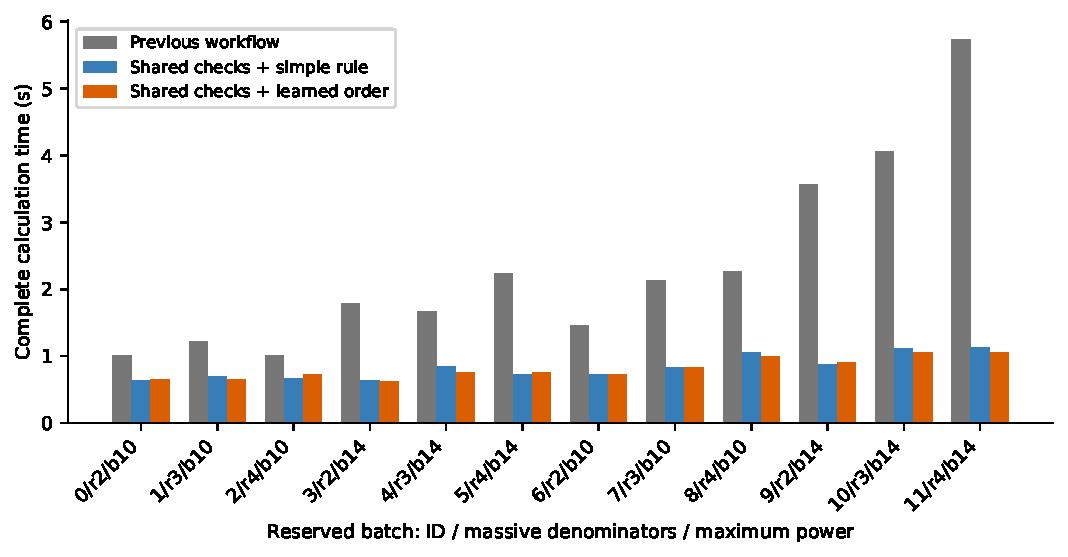
\includegraphics[width=\textwidth]{figures/batch_reuse_single.pdf}
 \caption{Median complete calculation time for the twelve reserved
 single-profile batches. All methods return the same exact reductions
 at loop orders one through twelve. The updated simple and learned
 routes share the improved exact checks and coefficient arithmetic.}
 \label{fig:batch-reuse-single}
\end{figure}
\begin{figure}[htbp]
 \centering
 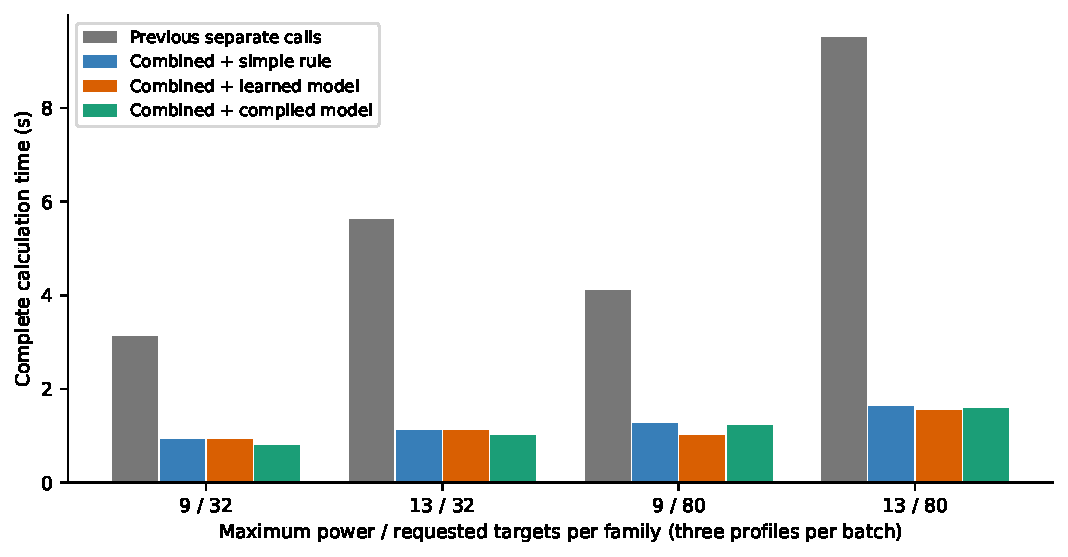
\includegraphics[width=\textwidth]{figures/batch_reuse_packed.pdf}
 \caption{Median complete time for the second reserved comparison.
 Each group contains three independent mass profiles. The previous
 route makes separate Kira calls; the other routes combine the selected
 systems. The target count on the axis is the requested count per
 profile and is capped by the available index vectors.}
 \label{fig:batch-reuse-packed}
\end{figure}
